\documentclass[lettersize,journal]{IEEEtran}

\usepackage{amsmath,amsfonts}
\usepackage{algorithmic}
\usepackage{algorithm}
\usepackage{array}
\usepackage[caption=false,font=normalsize,labelfont=sf,textfont=sf]{subfig}
\usepackage{textcomp}
\usepackage{stfloats}
\usepackage{url}
\usepackage{verbatim}
\usepackage{graphicx}
\usepackage{cite}
\usepackage{booktabs}
\usepackage{multirow}

\begin{document}

\title{Cross-Corpus and Cross-Task Depression Detection from Speech Using Frozen WavLM Representations}

\author{Mohammad~Ilyas~and~Vikram~Singh%
\thanks{Mohammad Ilyas is with the Department of Computer Science and Engineering, Moradabad Institute of Technology, Moradabad, Uttar Pradesh, India (e-mail: mohd.passion.cse@mitmoradabad.edu.in). Corresponding author: Mohammad Ilyas.}%
\thanks{Vikram Singh is with the Department of Computer Engineering, National Institute of Technology, Kurukshetra, Haryana, India (e-mail: viks@nitkkr.ac.in).}%
\thanks{ORCID identifiers are not available for either author. No IEEE membership status is claimed.}}

\markboth{IEEE Transactions on Computational Social Systems,~Vol.~XX, No.~XX, 2026}%
{Ilyas \MakeLowercase{\textit{et al.}}: Cross-Corpus and Cross-Task Depression Detection from Speech}

\maketitle

\begin{abstract}
Speech is a non-invasive behavioral signal that may reflect affective, psychomotor and cognitive changes, but depression classifiers trained in one corpus can be sensitive to language, recording conditions, elicitation task and label definition \cite{leal2025survey,morenoTorres2012datasetShift,alghowinem2016crossCultural}. We evaluated whether frozen self-supervised WavLM representations preserved depression-related information across corpora and speech tasks, and whether transfer failures reflected representation failure or classifier-boundary shift. In DAIC-WOZ, we developed a leakage-controlled participant-level pipeline using 10-second participant-speech windows, frozen \texttt{microsoft/wavlm-base-plus}, transformer layer 9, temporal mean pooling, participant mean aggregation and balanced logistic regression. The frozen DAIC WavLM classifier achieved ROC-AUC 0.6412 in zero-shot transfer to Android interview speech, but both the 0.5 and frozen DAIC thresholds predicted every Android interview participant as negative. An Android-trained interview classifier using the same frozen representation achieved within-Android ROC-AUC 0.8675. Android reading speech showed a similar pattern: zero-shot DAIC-to-reading ROC-AUC was 0.5795 with all-negative thresholded predictions, whereas Android-trained reading evaluation achieved ROC-AUC 0.8796. In participant-coherent Android analysis, reading-to-interview and interview-to-reading transfer achieved ROC-AUCs of 0.8475 and 0.8501; pooled reading-and-interview training achieved ROC-AUCs of 0.9058 for reading and 0.9135 for interview speech. Frozen WavLM features therefore retained useful depression-related ranking information, while decision boundaries and probability scales remained corpus- and task-sensitive. These are research classification findings, not clinical validation; DAIC local test labels were provisional, Android labels reflected HC/PT group status rather than PHQ-8 labels, and no prospective deployment study was performed.
\end{abstract}

\begin{IEEEkeywords}
Depression detection; speech analysis; self-supervised learning; WavLM; cross-corpus evaluation; domain shift; cross-task transfer
\end{IEEEkeywords}

\section{Introduction}

From an IEEE Transactions on Computational Social Systems perspective, this work treats speech as a human behavioral signal whose computational representation can shift across language, elicitation task and dataset context. The study therefore emphasizes robustness, transfer and responsible interpretation of behavioral computing systems rather than clinical deployment.

Depression is a common mental-health condition with substantial personal, functional and public-health impact. The World Health Organization estimates that 5.7\% of adults globally experience depression, and the US Preventive Services Task Force frames adult depression screening as a primary-care question only when systems are available for diagnosis, treatment and follow-up \cite{who2025depression,uspstf2023depressionScreening}. Speech has long been studied as a behavioral modality that may reflect affective, psychomotor and cognitive changes associated with depressive states, including changes in rhythm, pauses, energy, voice quality and prosody \cite{leal2025survey,tao2023featureCorrelation}. Compared with questionnaire-only or clinician-administered assessments, speech-based analysis is attractive because it can be collected during ordinary interactions. However, speech models also raise important questions about label validity, clinical interpretation, privacy, bias, screening versus diagnosis and deployment governance \cite{who2021aiHealthEthics,nist2023aiRmf,nautsch2019gdprSpeech,kelly2019clinicalImpactAI}.

Earlier speech-based depression studies have used handcrafted acoustic, prosodic, timing and interaction features, including pitch or F0, energy, cepstral features such as MFCCs, voice quality, speaking rate, pause behavior and response latency \cite{leal2025survey,valstar2016avec,tao2023featureCorrelation}. These features can be interpretable, but they are often sensitive to recording setup, language, task design and annotation quality. More recently, self-supervised speech models have offered reusable representations trained from large-scale unlabeled audio \cite{baevski2020wav2vec2,chen2022wavlm,yang2021superb}. Frozen representations from such models can reduce the risk of overfitting small clinical datasets, and can support controlled comparisons between corpora and elicitation tasks.

The central challenge addressed here is not only whether a model performs well inside one dataset, but whether the representation and decision rule survive shifts between datasets. DAIC-WOZ and the Androids Corpus differ in language, elicitation, label definition and recording context \cite{gratch2014distress,valstar2016avec,tao2023androids}. DAIC-WOZ uses English clinical-interview speech and PHQ-8 binary labels \cite{gratch2014distress,valstar2016avec,kroenke2009phq8}, whereas Androids Corpus uses Italian speech with healthy-control versus depression-patient group labels \cite{tao2023androids}. These targets are related but not identical. A classifier trained on DAIC-WOZ may therefore fail externally even if its representation still ranks Android participants above chance.

This distinction motivates a careful separation between zero-shot external validation, target-domain threshold adaptation, target-domain calibration and target-domain classifier retraining. In many applied machine-learning settings, these protocols answer different questions: zero-shot evaluation tests direct transfer of the complete frozen model; threshold adaptation tests whether a score scale can be shifted; calibration tests probability mapping; and target-domain retraining tests whether the representation supports a new decision boundary \cite{morenoTorres2012datasetShift,niculescuMizil2005probabilities,vanCalster2019calibration}. For mental-health speech modeling, conflating these protocols can lead to overstated claims.

Speech task is another important source of variation. Interview speech may include spontaneous response patterns, conversational timing and participant-interviewer dynamics. Reading speech is more controlled and may reduce lexical and conversational variability, but it can also remove clinically informative interactive behavior \cite{tao2023androids,tao2023featureCorrelation,leal2025survey}. A representation that works across both tasks would be useful for robust measurement, while task-specific classifier boundaries would imply that representation transfer and classifier transfer must be evaluated separately.

This study developed and audited a reproducible sequence of experiments through DAIC-WOZ methodology development, DAIC-to-Android zero-shot evaluation, Android within-corpus evaluation, and participant-coherent Android reading/interview cross-task transfer. The central research argument is that frozen WavLM speech representations retain useful depression-related information across corpora and tasks, but classifier boundaries are sensitive to corpus and task conditions. Target-corpus training and pooled multi-task exposure substantially improved discrimination compared with direct zero-shot model transfer.

The following research gaps motivate the present study. First, depression-related acoustic patterns are difficult to separate from speaker-specific voice characteristics. Learned speech representations may encode affective or behavioral cues together with stable voiceprint information, including vocal-tract characteristics, accent, speaking style, microphone conditions and recording context. This creates a confounding risk: a model may appear to capture depression-related behavior while partly relying on speaker- or corpus-specific cues. Second, many speech-based depression studies evaluate models under a single elicitation condition. Spontaneous interview speech and read speech differ in linguistic planning, cognitive load, pause behavior, fluency and prosodic expressiveness, so a model trained or evaluated under one task may not generalize reliably to another.

Third, cross-corpus generalization remains limited because datasets differ in population, recording setup, elicitation protocol, label distribution, clinical assessment procedure and class balance. These differences can shift both the representation distribution and the classifier decision boundary, producing degraded transfer, poor calibration or inappropriate threshold behavior. Fourth, classification performance is often reported without clearly separating the effects of representation choice, participant-level aggregation, timing descriptors, task condition, threshold selection, calibration and corpus shift. A systematic evaluation framework is therefore needed to examine why a model succeeds or fails across within-corpus, cross-corpus and cross-task settings.

This study is guided by four research questions. \textbf{RQ1} asks how effectively frozen self-supervised WavLM speech representations and timing-based speech features support participant-level depression-related behavioral signal classification on DAIC-WOZ. \textbf{RQ2} examines which WavLM representation-design choices, particularly transformer-layer selection and participant-level aggregation strategy, influence DAIC-WOZ classification performance. \textbf{RQ3} evaluates the extent to which a DAIC-WOZ-trained WavLM classifier transfers to Androids Corpus speech, and what threshold adaptation, score calibration and target-domain classifier learning reveal about calibration and classifier-boundary shift. \textbf{RQ4} investigates how Android reading and interview task conditions affect within-corpus, cross-task and pooled-task depression-related behavioral signal modeling.

The study contributes a structured evaluation framework for depression-related speech modeling that separates representation selection, participant-level aggregation, timing descriptors, cross-corpus transfer, calibration behavior and cross-task generalization. Rather than presenting the model as a clinical diagnostic tool, the analysis focuses on how speech-based behavioral representations behave under dataset and task shifts. The contributions are:

\begin{itemize}
\item An empirical DAIC-WOZ evaluation of frozen WavLM and timing-based participant-level behavioral signal classification, aligned with RQ1.
\item Analysis of WavLM layer selection and participant aggregation choices on DAIC-WOZ, aligned with RQ2.
\item DAIC-to-Android transfer evaluation with threshold, calibration and target-domain classifier-boundary diagnosis, aligned with RQ3.
\item Within-Android reading/interview benchmarks, participant-coherent cross-task transfer and pooled-task evaluation, aligned with RQ4.
\item A reproducible experiment registry with paper-claim safeguards.
\end{itemize}

Overall, the evaluation findings indicate that depression-related speech modeling is strongly affected by representation choice, participant-level aggregation, timing and prosodic information, task condition, and corpus shift. The DAIC-WOZ experiments show that frozen WavLM representations and timing descriptors capture useful but limited depression-related behavioral cues, whereas the Androids Corpus experiments reveal that direct cross-corpus transfer is constrained by calibration mismatch, threshold instability, and classifier-boundary shift. The cross-task analysis further suggests that reading and interview speech share some transferable information but differ sufficiently to affect model reliability. These observations connect directly with the identified research gaps and indicate that future work should focus on speaker-invariant or identity-aware representation learning, cross-corpus and cross-task adaptation, improved calibration strategies, and larger externally validated studies before such systems can be considered for clinically supervised decision-support research.

\section{Related Work}

\subsection{Speech-based depression detection}

Speech-based depression detection has been studied using clinical interviews, prompted responses, reading tasks and other elicitation paradigms \cite{leal2025survey}. The motivation is that depression may affect psychomotor behavior, speech timing, prosody, energy and voice quality. However, the direction and strength of reported markers are not uniform: acoustic findings can depend on sex, age, language, recording context, speech task and label definition, making cross-study comparison difficult \cite{leal2025survey}. This heterogeneity is one reason the present study separates corpus, task and classifier-boundary questions rather than treating speech-depression performance as a single pooled benchmark.

\subsection{Physiological motivation for speech-based depression analysis}

Human speech is produced through coordinated respiratory, phonatory, resonatory and articulatory processes. Airflow from the lungs provides respiratory drive; vocal-fold vibration in the larynx generates the acoustic source; and the vocal tract shapes this source through resonance and articulation. In source-filter terms, variation in vocal-fold vibration, subglottal pressure, articulatory precision and vocal-tract configuration can influence measurable properties such as fundamental frequency, intensity, formant structure, spectral balance and voice quality. These properties correspond to feature families commonly used in affective speech analysis, including pitch or F0, energy, cepstral and spectral descriptors, formant or voice-quality measures, pause duration and speaking rate \cite{leal2025survey,valstar2016avec,tao2023featureCorrelation}.

Depression-related speech analysis is motivated because mood, psychomotor activity, emotional expressivity, cognitive effort and physiological arousal can influence how speech is planned and produced. Prior speech-depression studies have reported patterns such as reduced pitch variability, lower energy, slower articulation, longer pauses, flatter intonation, breathier voice quality and less regular timing, although findings vary across speakers, languages, tasks and recording conditions \cite{leal2025survey,tao2023featureCorrelation}. These patterns should not be treated as diagnostic markers by themselves. They are task- and population-dependent behavioral signals, and the present study evaluates corpus labels under controlled research protocols rather than clinical diagnosis.

This rationale also motivates comparing handcrafted features with self-supervised representations. Handcrafted descriptors measure specific vocal properties, while WavLM embeddings may encode broader combinations of phonatory, prosodic, spectral and temporal information learned from speech pretraining \cite{chen2022wavlm,yang2021superb}. In this study, WavLM is used as a frozen representation to test whether depression-related speech information transfers across corpus and task conditions, not as a standalone clinical model.

\subsection{Handcrafted acoustic and timing features}

Handcrafted features remain important because they provide interpretable links to speech production and interaction behavior. Common categories include pitch or F0, intensity and energy, spectral or cepstral measures such as MFCCs, formant or voice-quality features, pause duration, speech rate and turn-taking or response-latency measures \cite{leal2025survey,valstar2016avec,tao2023featureCorrelation}. In DAIC-WOZ-style guided interviews, response latency and participant-turn timing may be informative because they preserve aspects of the original interview timeline. Feature toolkits used in affective-computing benchmarks, including COVAREP/openSMILE-style low-level descriptors and functionals, reflect this tradition of interpretable acoustic and prosodic measurement \cite{valstar2016avec,leal2025survey}. These features may not transfer directly to corpora lacking compatible interviewer and participant timing annotations.

\subsection{Self-supervised speech representations}

Self-supervised speech models learn representations from large unlabeled speech corpora and can be used as frozen feature extractors or fine-tuned for downstream tasks \cite{baevski2020wav2vec2,chen2022wavlm,yang2021superb}. WavLM is one such model family designed to produce general-purpose speech representations \cite{chen2022wavlm}. Benchmarking work such as SUPERB uses shared pretrained encoders with lightweight downstream heads, while depression-speech studies have explored wav2vec 2.0 or related SSL representations as feature extractors or fine-tuned encoders \cite{yang2021superb,wu2023sslDepression,huang2024voicePretraining}. In small mental-health datasets, frozen encoders can provide a conservative first baseline because they avoid adapting millions of parameters to limited labels. However, SSL pretraining does not by itself establish domain invariance or clinical validity.

\subsection{Cross-corpus depression detection}

Cross-corpus depression detection evaluates whether a model developed on one dataset transfers to another. This is especially important because clinical speech corpora differ in language, microphone conditions, participant recruitment, label source, task design and class prevalence \cite{alghowinem2016crossCultural,seneviratne2021generalized,leal2025survey}. Prior cross-cultural and cross-database depression-speech work motivates the question but does not remove the need to label each transfer protocol precisely. A zero-shot result measures the complete source-trained model, while target-domain training measures whether the feature representation remains useful when a new classifier boundary is learned.

\subsection{Reading versus spontaneous speech}

Reading and spontaneous interview speech may capture overlapping but non-identical information. Reading constrains lexical content and can reduce conversational variability, whereas interview speech may include spontaneous fluency, turn-taking and response latency \cite{tao2023androids,tao2023featureCorrelation,leal2025survey}. The Androids Corpus was designed with both read and spontaneous/interview recordings, including paired participants, which permits a direct comparison of these tasks \cite{tao2023androids}. Participant-level leakage safeguards are essential when the same person contributes both tasks.

\subsection{Domain shift, calibration and transfer}

Dataset shift can affect feature distributions, class priors and conditional label relationships, and can therefore alter both score calibration and the decision boundary implied by a source-trained classifier \cite{morenoTorres2012datasetShift}. A classifier can show above-chance ranking under ROC-AUC while failing at a fixed threshold if the probability scale shifts. Calibration assesses whether predicted probabilities correspond to observed outcome frequencies and is distinct from discrimination; Brier score, calibration slope/intercept, Platt scaling, isotonic regression and temperature scaling are common tools for this question \cite{brier1950probabilityForecasts,niculescuMizil2005probabilities,guo2017calibration,vanCalster2019calibration}. Calibration can improve probability scores without improving ranking, and threshold adaptation can improve thresholded metrics without demonstrating pure zero-shot transfer. For this reason, this paper reports protocol scope explicitly for each result.

\section{Datasets and Experimental Design}

\subsection{Study design}

The study followed a sequential Phase 1-2E design. Phase 1 developed and froze DAIC-WOZ research candidates. Phase 1A established participant-level metadata and final-layer WavLM baselines. Phase 1B compared WavLM transformer layers using DAIC training data only and selected layer 9. Phase 1C compared participant-level aggregation methods for layer 9 and retained arithmetic mean aggregation. Phase 1D evaluated speech-timing features and early fusion, while Phase 1E evaluated late fusion. Phase 1F evaluated the frozen DAIC candidates once on a provisional local labeled DAIC test split.

Phase 2 moved to Androids Corpus preparation and external-compatibility testing. Phase 2A audited the Android data and established that WavLM preprocessing for Candidate A could be reproduced, while the DAIC timing model could not be directly transferred because only 17 of 28 timing features were exactly compatible. Phase 2B applied the frozen DAIC WavLM classifier zero-shot to Android interview speech. Phase 2C diagnosed whether failure came from threshold shift, calibration shift or classifier-boundary shift. Phase 2D evaluated Android reading speech. Phase 2E used participant-coherent folds across paired reading and interview tasks to evaluate cross-task transfer and pooled-task training.

\begin{figure*}[!t]
\centering
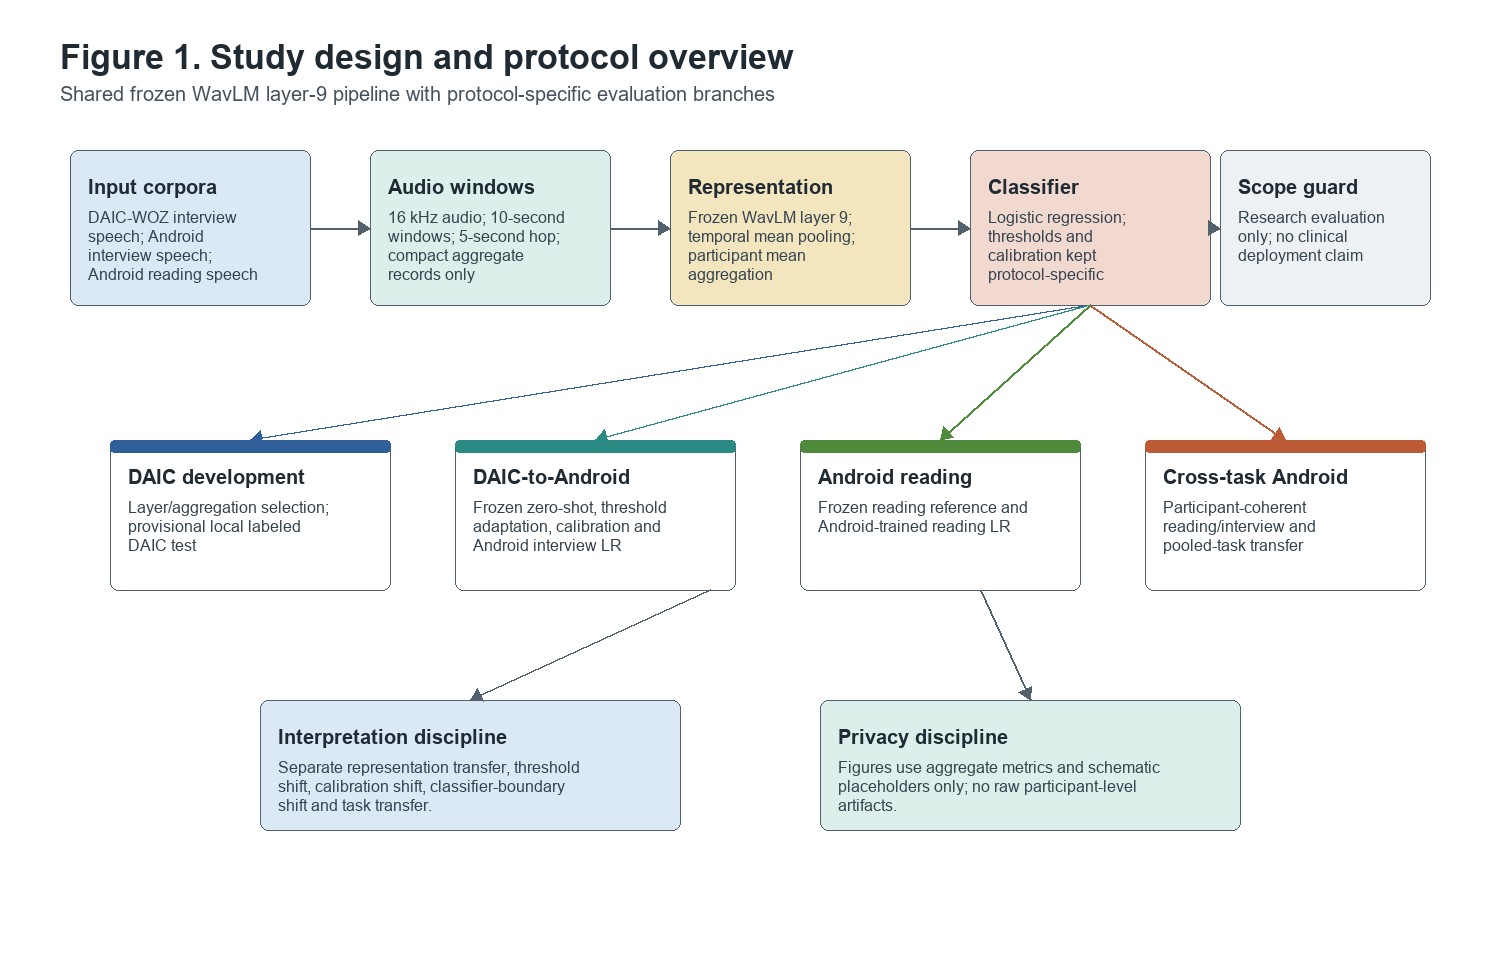
\includegraphics[width=0.95\textwidth]{figures/figure1_study_design_protocol_overview.png}
\caption{Study design and protocol overview for the frozen WavLM layer-9 participant-level research pipeline. The schematic distinguishes DAIC-WOZ development, DAIC-to-Android interview transfer, Android reading evaluation and participant-coherent Android cross-task transfer.}
\label{fig:study-design}
\end{figure*}

\subsection{Datasets}

\subsubsection{DAIC-WOZ}

The DAIC-WOZ Phase 1 clean dataset contained 187 usable participants after excluding participants 409 and 422. The official development split used here contained 106 training, 34 development and 47 local labeled test participants. The corresponding 10-second clean speech-window counts were 9,001 train, 3,314 development and 4,743 local labeled test windows, for 17,058 total windows. Labels were \texttt{PHQ8\_Binary} labels derived from PHQ-8 questionnaire scoring \cite{valstar2016avec,kroenke2009phq8}. The test split used in Phase 1F was a provisional local labeled test derived from \texttt{Data/full\_test\_split.csv}; official AVEC hidden-test provenance was not established. Therefore, DAIC test results are described as provisional local labeled test results rather than official hidden AVEC test performance.

\subsubsection{Androids Corpus}

The Androids Corpus audit identified 118 unique participants, with 54 healthy controls and 64 depression patients \cite{tao2023androids}. The corpus contained 116 full interview recordings, 112 read-speech recordings and 874 interview clips. Reading recordings included 54 HC and 58 PT participants; interview recordings included 52 HC and 64 PT participants. A total of 110 participants had both reading and interview recordings, with 52 HC and 58 PT participants in the paired Phase 2E subset. Android labels were treated as clinical group status labels, not PHQ-8 labels: HC was encoded as 0 and PT as 1. The Android speech was Italian \cite{tao2023androids}, and Android evaluation used task-specific folds for Phase 2C and Phase 2D, then participant-coherent reading/interview folds for Phase 2E.

\begin{table*}[!t]
\caption{Dataset and task summary}
\label{tab:dataset-task-summary}
\centering
\scriptsize
\setlength{\tabcolsep}{3pt}
\renewcommand{\arraystretch}{1.15}
\resizebox{\textwidth}{!}{%
\begin{tabular}{lllllll}
\toprule
Corpus & Task & Participants & Class counts & Recordings/windows & Language & Evaluation role \\
\midrule
DAIC-WOZ Phase 1 clean & Interview participant speech & 187 & Train/dev/local test labels from PHQ8\_Binary & 17,058 clean 10-second windows & English & Representation development and provisional local testing \\
Androids Corpus & Interview & 116 & HC=52, PT=64 & 116 full recordings; 4,249 valid windows in Phase 2B/2C & Italian & Zero-shot external evaluation and within-Android interview benchmark \\
Androids Corpus & Reading & 112 & HC=54, PT=58 & 112 recordings; 955 valid windows & Italian & Reading zero-shot and within-Android reading benchmark \\
Androids Corpus & Paired reading/interview & 110 & HC=52, PT=58 & Paired participant-level reading and interview embeddings & Italian & Participant-coherent cross-task and pooled-task analysis \\
\bottomrule
\end{tabular}%
}
\begin{minipage}{0.96\textwidth}
\vspace{2pt}
\footnotesize DAIC-WOZ denotes the Distress Analysis Interview Corpus--Wizard-of-Oz; HC denotes healthy control and PT denotes patient group labels in the Androids Corpus. Android labels are HC/PT group labels rather than PHQ-8 labels.
\end{minipage}
\end{table*}


\section{Methods}

\subsection{Speech Preprocessing}

DAIC preprocessing used participant-only speech intervals from the clinical interview. Participant speech was reconstructed from clean mapped intervals, converted to mono, resampled to 16 kHz, corrected for DC offset and peak-normalized without dataset-level normalization. Ten-second windows with 50\% overlap were used, equivalent to a 5-second hop and 160,000 samples per full window. Incomplete windows shorter than 10 seconds were not used for WavLM extraction. The completed extraction used no data augmentation and no denoising.

Android interview and reading processing preserved task separation. Android interview processing reconstructed participant speech where compatible with Phase 2A timing and clip audits, while Android reading used full reading recordings. Phase 2D reading extraction used the same 16 kHz target sample rate, 10-second windows, 5-second hop, DC-offset removal and peak normalization. The reading extraction report explicitly recorded no dataset normalization, no augmentation and no denoising. Reading and interview speech were not combined before Phase 2E pooled-task model training; pooled-task training combined participant-level examples under participant-coherent folds rather than concatenating a participant's tasks into a single feature vector.

\subsection{WavLM representation}

WavLM is a pretrained self-supervised speech model using masked speech prediction and denoising-oriented pretraining for broad speech representation learning \cite{chen2022wavlm}. All WavLM experiments used \texttt{microsoft/wavlm-base-plus} pinned to model commit \texttt{4c66d4806a428f2e922ccfa1a962776e232d487b}. The encoder was frozen and used in evaluation/inference mode. Phase 1B inspected hidden-state indexing and compared the 12 transformer encoder layers. The primary selected representation was transformer layer 9, not the pre-transformer feature-projection state. Each 10-second window was represented by temporal mean pooling over the WavLM time dimension, producing a 768-dimensional vector. Participant-level representations were produced by arithmetic mean pooling across valid window embeddings.

Layer 9 and mean participant aggregation were selected using DAIC development experiments only. Android results were not used to select the WavLM layer or participant aggregation method.

\subsection{Classifiers}

The main classifier family was logistic regression with L2 regularization, \texttt{class\_weight="balanced"} and \texttt{max\_iter=10000}. WavLM-only pipelines used a \texttt{StandardScaler} followed by logistic regression. Timing models used training-fold imputation and scaling. Hyperparameter selection considered C values of 0.0001, 0.001, 0.01, 0.1, 1.0, 10.0 and 100.0. Scalers, imputers, calibrators and classifiers were fit inside the appropriate training folds only. Thresholds were selected from training or development data as specified by each protocol, and threshold-adapted results were not described as pure zero-shot evaluation.

\subsection{Evaluation protocols}

\subsubsection{DAIC development and provisional local testing}

DAIC development used train-only or train/development protocols depending on phase. Phase 1B through Phase 1E model-selection comparisons used training-data cross-validation and development evaluation where specified. Phase 1F evaluated frozen DAIC candidates once on 47 provisional local labeled test participants. This Phase 1F test was not treated as official hidden AVEC evaluation.

\subsubsection{DAIC-to-Android zero-shot evaluation}

Phase 2B applied the frozen DAIC WavLM Candidate A directly to Android interview participant embeddings. The source corpus was DAIC-WOZ, the target corpus was Androids Corpus, the source task was free-speech-compatible interview speech and the target task was Android interview speech. No Android labels were used for model fitting, scaler fitting, threshold selection, calibration or model revision. This was the main zero-shot external evaluation.

\subsubsection{Threshold-only adaptation}

Phase 2C Protocol B preserved the frozen DAIC score ranking but selected thresholds within Android training folds. This used Android target labels for threshold selection and therefore was target-domain threshold adaptation, not pure zero-shot evaluation. The classifier was not refitted, and the protocol did not change individual predicted probabilities. Under dataset-shift terminology, it tested whether a source score could be made operational under a target-domain threshold rather than whether the source classifier transferred unchanged \cite{morenoTorres2012datasetShift}.

\subsubsection{Frozen-score calibration}

Phase 2C Protocol C calibrated frozen DAIC scores using Android training folds. This used target-domain labels to fit calibration mappings and therefore was target-domain score calibration rather than zero-shot evaluation. The WavLM encoder and source score generator were not refit. This protocol addressed probability calibration, not representation learning or source-model external validation \cite{niculescuMizil2005probabilities,vanCalster2019calibration}.

\subsubsection{Android within-corpus interview evaluation}

Phase 2C Protocol D trained a logistic-regression classifier within Android interview folds using the same frozen layer-9 participant mean representation. Target labels were used for training, inner hyperparameter selection and fold-specific threshold adaptation. This protocol tested within-Android discrimination, not DAIC-to-Android model transfer.

\subsubsection{Android within-corpus reading evaluation}

Phase 2D evaluated reading speech separately from interview speech. Protocol A applied the frozen DAIC WavLM classifier zero-shot to Android reading embeddings. Protocol B trained an Android reading logistic-regression classifier under participant-level nested five-fold cross-validation using the same frozen layer-9 mean representation. The Android-trained reading result was within-corpus validation, not external validation.

\subsubsection{Participant-coherent cross-task transfer}

Phase 2E created participant-coherent folds over the 110 Android participants with both reading and interview recordings. Matched-task protocols trained and evaluated on the same task. Cross-task protocols trained on one task and evaluated on the other task for held-out participants. Participants did not cross training and evaluation folds, and reading/interview examples from the same participant remained in the same fold.

\subsubsection{Pooled-task training}

Phase 2E pooled reading and interview training examples within participant-coherent folds and evaluated separately on reading and interview held-out participants. Pooled training used the same frozen layer-9 representation and logistic-regression model family. Pooled results were within-Android pooled-task estimates, not cross-corpus external validation.

\subsection{Leakage prevention}

All model evaluation was participant-level. Cross-validation used participant grouping, and the outer evaluation fold was isolated from preprocessing, hyperparameter selection and threshold selection. \texttt{StandardScaler} fitting occurred inside training folds only. C selection used inner folds only. Threshold selection used training out-of-fold predictions or development data according to the protocol, never the held-out fold being evaluated. Phase 2E introduced participant-coherent folds so that reading and interview recordings from the same participant remained together.

\subsection{Metrics and uncertainty}

Primary discrimination was reported with ROC-AUC. Additional metrics included PR-AUC, balanced accuracy, macro F1, positive-class precision, sensitivity, specificity, negative predictive value and Brier score. Brier score was used as a proper scoring-rule summary of probability error, while discrimination and calibration were interpreted separately \cite{brier1950probabilityForecasts,vanCalster2019calibration}. Balanced accuracy is also interpretable as unweighted average recall. Bootstrap uncertainty estimates used 5,000 stratified participant-level bootstrap replicates where reported. Confidence intervals for Phase 2E paired comparisons were treated as exploratory because repeated cross-validation and paired task protocols induce dependencies.

\subsection{Reproducibility and experiment governance}

The repository preserved frozen protocols, source-code configurations, compact run records and an experiment registry. The frozen source tag for this manuscript was \texttt{paper-experiment-freeze-v1}. The registry contained 42 completed experiment or audit records and explicit paper-interpretation metadata distinguishing methodological ablations, provisional local test results, zero-shot external evaluations, target-domain adaptation and within-corpus validation. Registry validation was read-only, and compact records excluded restricted artifacts such as raw audio, embeddings, participant predictions and fitted models.

\section{Results}

Tables 2-6 summarize the numerical results and result-scope caveats. Figures 2-5 visualize the main DAIC development, DAIC-to-Android adaptation, Android task-transfer and domain-shift findings.

\subsection{DAIC representation development}

The DAIC development results address RQ1 and RQ2 by comparing frozen WavLM representations, timing descriptors, layer selection and participant-level aggregation under leakage-controlled participant protocols.

Phase 1A established initial participant-level baselines. The metadata-only sanity baseline achieved train-CV ROC-AUC 0.5510 and provisional local test ROC-AUC 0.4437. The final-layer WavLM participant baseline achieved train-CV ROC-AUC 0.5115, development ROC-AUC 0.5692 and provisional local test ROC-AUC 0.5195. These early results motivated a frozen layer-wise representation analysis.

Phase 1B evaluated all 12 WavLM transformer layers using DAIC train-only nested cross-validation. Layer 9 had the strongest mean outer ROC-AUC, 0.5956, compared with 0.4988 for layer 12. Layer 9 was therefore selected for subsequent WavLM experiments. This selection used DAIC training data only and did not use Android results.

Phase 1C tested whether participant aggregation limited performance. Mean aggregation for layer 9 achieved mean outer ROC-AUC 0.5956, median aggregation achieved 0.5905 and mean-plus-standard-deviation aggregation with PCA achieved 0.5683. Because alternatives did not improve train-only performance, arithmetic mean aggregation was retained.

Phase 1D examined whether compact speech-timing features captured information lost by concatenating participant speech intervals. Timing-only features achieved train nested-CV ROC-AUC 0.6126, WavLM-only achieved 0.5956 and early fusion achieved 0.5747. Phase 1E then compared timing-only, WavLM-only and late-fusion protocols; timing-only remained strongest among these DAIC guided-interview comparisons, while weighted late fusion and logistic stacking did not improve the final candidate.

Phase 1F froze two DAIC research candidates. Candidate A was the free-speech-compatible WavLM layer-9 mean representation with C=0.001 and frozen threshold 0.5558; it achieved provisional local test ROC-AUC 0.5065. Candidate B was the guided-interview timing model with C=100.0 and frozen threshold 0.2927; it achieved provisional local test ROC-AUC 0.6775. Candidate B was not directly portable to Android because Android timing features were not fully compatible with the Phase 1 timing definitions.

\begin{figure*}[!t]
\centering
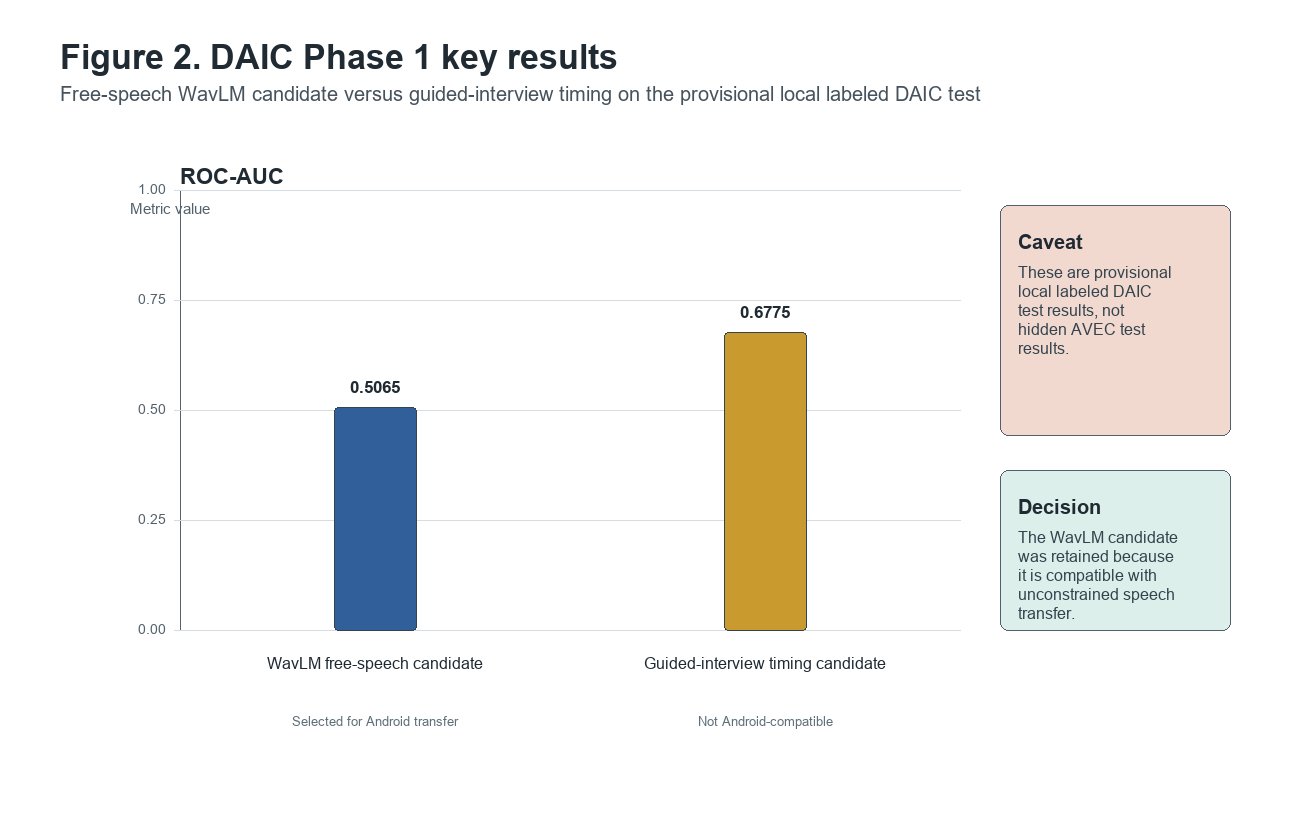
\includegraphics[width=0.95\textwidth]{figures/figure2_daic_phase1_key_results.png}
\caption{DAIC Phase 1F provisional local labeled test ROC-AUC for the frozen WavLM free-speech candidate and the guided-interview timing candidate. The WavLM candidate is lower on this DAIC-only local split but was retained for Android transfer because it is compatible with unconstrained speech; the timing candidate depends on guided-interview timing definitions.}
\label{fig:daic-phase1}
\end{figure*}

\begin{table*}[!t]
\caption{DAIC development results}
\label{tab:daic-development}
\centering
\scriptsize
\setlength{\tabcolsep}{3pt}
\renewcommand{\arraystretch}{1.15}
\resizebox{\textwidth}{!}{%
\begin{tabular}{llllll}
\toprule
Phase & Result & Scope & Primary metric & ROC-AUC & Notes \\
\midrule
1A & Metadata-only sanity baseline & Provisional local labeled test & Test ROC-AUC & 0.4437 & Duration/window count nearly redundant; sanity baseline only \\
1A & Final-layer WavLM baseline & Provisional local labeled test & Test ROC-AUC & 0.5195 & Baseline before layer-wise analysis \\
1B & Layer 9 WavLM & Train-only nested CV & Mean outer ROC-AUC & 0.5956 & Selected layer using DAIC training data only \\
1B & Layer 12 WavLM & Train-only nested CV & Mean outer ROC-AUC & 0.4988 & Final transformer layer comparison \\
1C & Layer-9 mean aggregation & Train-only nested CV & Mean outer ROC-AUC & 0.5956 & Retained participant mean aggregation \\
1C & Layer-9 median aggregation & Train-only nested CV & Mean outer ROC-AUC & 0.5905 & Not selected \\
1C & Layer-9 mean plus std with PCA & Train-only nested CV & Mean outer ROC-AUC & 0.5683 & Not selected \\
1D & Timing-only & Train-only nested CV & Mean outer ROC-AUC & 0.6126 & Stronger in DAIC guided-interview setting \\
1D & WavLM-only & Train-only nested CV & Mean outer ROC-AUC & 0.5956 & Locked free-speech representation \\
1D & Early fusion & Train-only nested CV & Mean outer ROC-AUC & 0.5747 & Did not improve \\
1E & Weighted late fusion & Train-only nested CV & Mean outer ROC-AUC & 0.6044 & Did not exceed timing-only \\
1E & Logistic stacking & Train-only nested CV & Mean outer ROC-AUC & 0.5413 & Not selected \\
1F & Frozen WavLM Candidate A & Provisional local labeled test & Test ROC-AUC & 0.5065 & Free-speech-compatible candidate \\
1F & Frozen timing Candidate B & Provisional local labeled test & Test ROC-AUC & 0.6775 & Guided-interview timing candidate; not Android-compatible \\
\bottomrule
\end{tabular}%
}
\begin{minipage}{0.96\textwidth}
\vspace{2pt}
\footnotesize Phase 1B/1C values are train-only nested cross-validation estimates. Phase 1F values are provisional local labeled DAIC test results, not official hidden AVEC test results.
\end{minipage}
\end{table*}


\subsection{Zero-shot DAIC-to-Android interview transfer}

This experiment addresses RQ3 by testing direct source-model transfer from DAIC-WOZ to Android interview speech before any target-domain thresholding, calibration or classifier retraining.

Phase 2B applied the frozen DAIC WavLM Candidate A to 116 Android interview participants, including 52 HC and 64 PT participants. The Android interview preprocessing produced 4,249 valid 10-second windows and the embedding quality checks passed. The frozen DAIC classifier achieved zero-shot ROC-AUC 0.6412 and PR-AUC 0.6809. However, predicted probabilities were compressed below both the default 0.5 threshold and the frozen DAIC threshold of 0.5558: the maximum predicted probability was 0.3938, and every participant was predicted negative at both thresholds. Thresholded balanced accuracy was 0.5000, macro F1 was 0.3095, sensitivity was 0.0000 and specificity was 1.0000. The Brier score was 0.4056.

This result indicates limited cross-corpus ranking transfer, not successful thresholded classification.

\begin{table*}[!t]
\caption{Cross-corpus Android interview results}
\label{tab:android-interview-transfer}
\centering
\scriptsize
\setlength{\tabcolsep}{3pt}
\renewcommand{\arraystretch}{1.15}
\resizebox{\textwidth}{!}{%
\begin{tabular}{llllllllll}
\toprule
Protocol & Training data & Target labels used? & Classifier refit? & ROC-AUC & PR-AUC & Brier & Balanced accuracy & Macro F1 & Interpretation \\
\midrule
Frozen DAIC zero-shot at 0.5 & DAIC-WOZ & No & No & 0.6412 & 0.6809 & 0.4056 & 0.5000 & 0.3095 & Limited ranking transfer; all-negative predictions \\
Frozen DAIC zero-shot at frozen threshold & DAIC-WOZ & No & No & 0.6412 & 0.6809 & 0.4056 & 0.5000 & 0.3095 & Same all-negative decision outcome \\
Threshold-only adaptation & DAIC-WOZ scores plus Android train-fold thresholds & Yes, thresholds only & No & 0.6412 & 0.6809 & 0.4056 & 0.5733 & 0.5688 & Target-domain threshold adaptation, not zero-shot \\
Frozen-score calibration & DAIC-WOZ scores plus Android train-fold calibration & Yes, calibration only & No source classifier refit & 0.5694 & 0.6001 & 0.2474 & 0.5883 & 0.5857 & Improved Brier score but not ranking \\
Android-trained interview LR & Android interview folds & Yes & Yes & 0.8675 & 0.8892 & 0.1695 & 0.8275 & 0.8263 & Strong within-Android discrimination \\
\bottomrule
\end{tabular}%
}
\begin{minipage}{0.96\textwidth}
\vspace{2pt}
\footnotesize Protocols using Android labels for threshold adaptation or calibration are target-domain adaptation protocols, not pure zero-shot evaluation. Android-trained logistic regression is within-Android evaluation, not external validation.
\end{minipage}
\end{table*}


\subsection{Domain-shift diagnosis}

This analysis extends RQ3 by separating discrimination, threshold placement, probability calibration and target-domain classifier learning on the same Android interview representation.

Phase 2C separated threshold shift, calibration shift and classifier-boundary shift on the same 116 Android interview participants. Protocol A reproduced the frozen DAIC zero-shot ROC-AUC of 0.6412. Protocol B used Android training folds for threshold-only adaptation and preserved ROC-AUC 0.6412 while improving macro F1 to 0.5688. Protocol C calibrated frozen DAIC scores using Android training folds; Brier score improved to 0.2474, but ROC-AUC decreased to 0.5694. Protocol D trained an Android interview logistic-regression classifier on the same frozen layer-9 participant embeddings and achieved ROC-AUC 0.8675, PR-AUC 0.8892, balanced accuracy 0.8275 and macro F1 0.8263 with fold-specific threshold adaptation. The Phase 2C protocols therefore separate discrimination, thresholded classification and probability calibration rather than treating all improvements as external transfer \cite{niculescuMizil2005probabilities,vanCalster2019calibration}.

The Android-trained interview classifier improved ROC-AUC over the frozen DAIC reference by 0.2263. Feature-distribution analysis showed a centroid cosine distance of 0.1767, mean absolute standardized shift of 2.3116 and 550 of 768 features shifted by more than one DAIC standard deviation. Together, these findings indicate that classifier-boundary shift was the dominant failure source, while threshold and calibration shifts were secondary.

\begin{figure*}[!t]
\centering
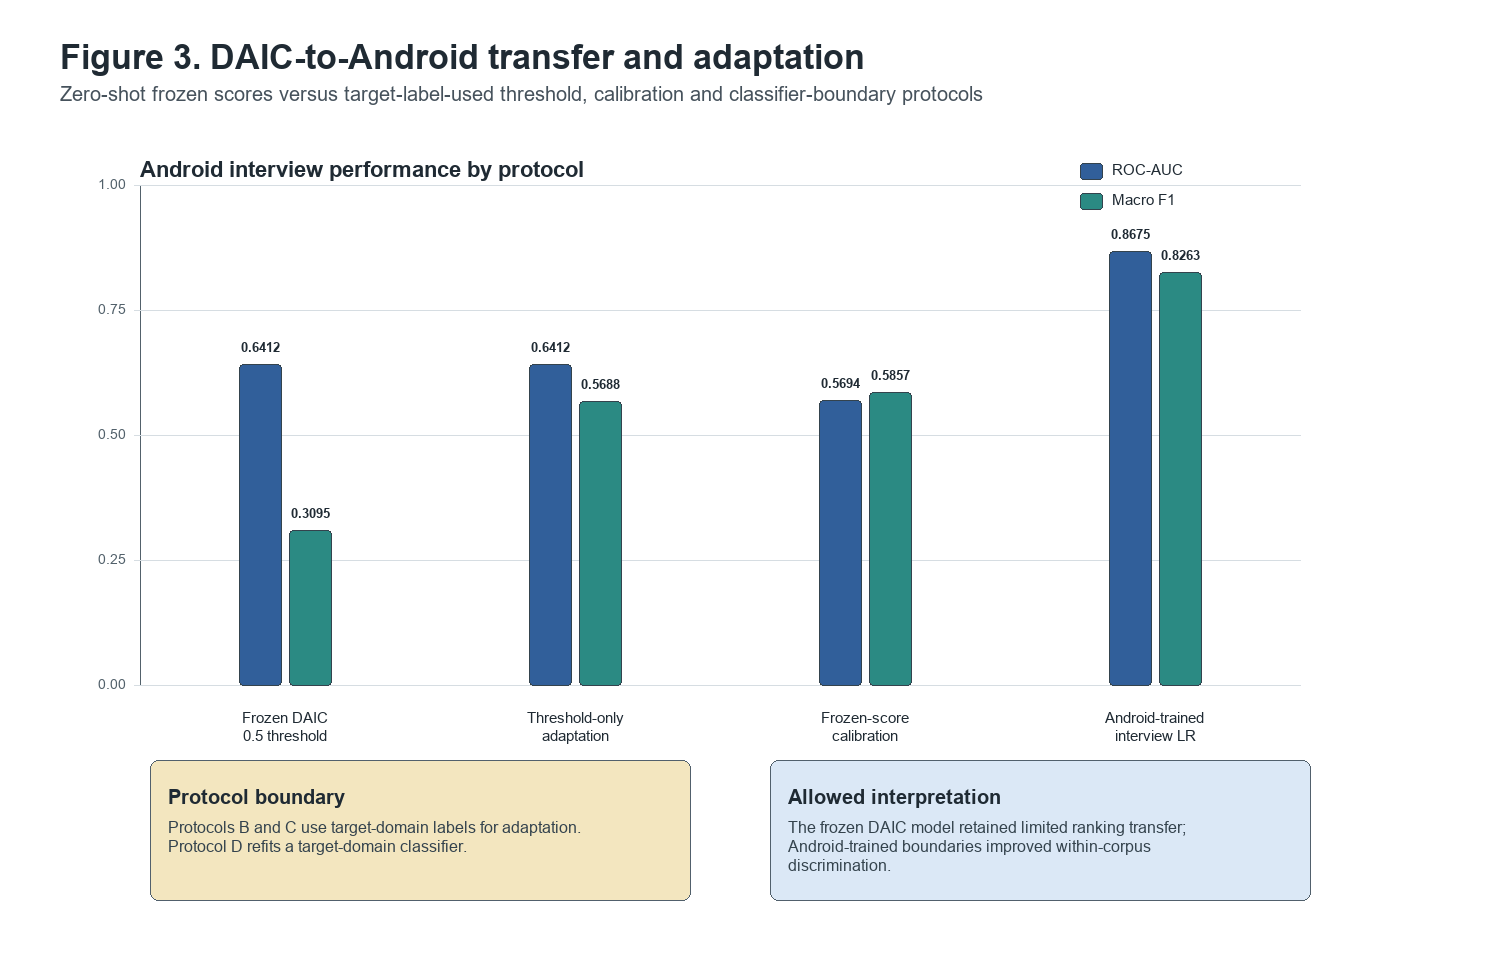
\includegraphics[width=0.95\textwidth]{figures/figure3_daic_android_transfer_adaptation.png}
\caption{Android interview protocol comparison for frozen DAIC zero-shot scores, threshold-only adaptation, frozen-score calibration and Android-trained logistic regression. ROC-AUC and macro F1 are plotted from \texttt{records/runs/phase2c\_20260703\_125614/phase2c\_protocol\_comparison.csv}.}
\label{fig:transfer-adaptation}
\end{figure*}

\subsection{Android reading-speech evaluation}

The Android reading analysis contributes to RQ4 by evaluating whether the same frozen representation supports a more constrained speech task, while also testing the DAIC-trained classifier under a second Android target condition.

Phase 2D evaluated 112 Android reading participants, including 54 HC and 58 PT participants. Reading preprocessing produced 955 valid 10-second windows with zero extraction failures, and participant aggregation used all 955 windows.

The frozen DAIC WavLM classifier transferred less strongly to reading speech than to Android interview speech, with zero-shot ROC-AUC 0.5795 and PR-AUC 0.5997. As in interview transfer, all participants were predicted negative at both the 0.5 threshold and the frozen DAIC threshold. In contrast, the Android-trained reading classifier achieved ROC-AUC 0.8796 with 95\% CI [0.8113, 0.9377], PR-AUC 0.8929, balanced accuracy 0.7768, macro F1 0.7766 and Brier score 0.1438. This was a within-Android nested cross-validation estimate, not external validation.

\begin{table*}[!t]
\caption{Android reading results}
\label{tab:android-reading}
\centering
\scriptsize
\setlength{\tabcolsep}{3pt}
\renewcommand{\arraystretch}{1.15}
\resizebox{\textwidth}{!}{%
\begin{tabular}{lllllllllll}
\toprule
Protocol & Training data & Participants & Windows & ROC-AUC & 95\% CI & PR-AUC & Brier & Balanced accuracy & Macro F1 & Interpretation \\
\midrule
Frozen DAIC zero-shot reading & DAIC-WOZ & 112 & 955 & 0.5795 & Not reported & 0.5997 & 0.3351 & 0.5000 & 0.3253 & All participants predicted negative \\
Android-trained reading LR & Android reading folds & 112 & 955 & 0.8796 & [0.8113, 0.9377] & 0.8929 & 0.1438 & 0.7768 & 0.7766 & Within-Android reading benchmark \\
\bottomrule
\end{tabular}%
}
\begin{minipage}{0.96\textwidth}
\vspace{2pt}
\footnotesize The Android-trained row is within-corpus validation and not independent external validation.
\end{minipage}
\end{table*}


\subsection{Reading-versus-interview comparison}

The Phase 2D descriptive task comparison contrasted Android-trained reading and interview classifiers. The reading classifier achieved ROC-AUC 0.8796, while the interview classifier from Phase 2C achieved ROC-AUC 0.8675. The task centroid cosine distance was 0.0442, and within-participant reading/interview cosine similarity averaged 0.9273 across 110 participants with both tasks. Nevertheless, 292 of 768 features shifted by more than one interview standard deviation. Because the original reading and interview task folds differed, this comparison was descriptive rather than a controlled cross-task transfer test.

\begin{figure*}[!t]
\centering
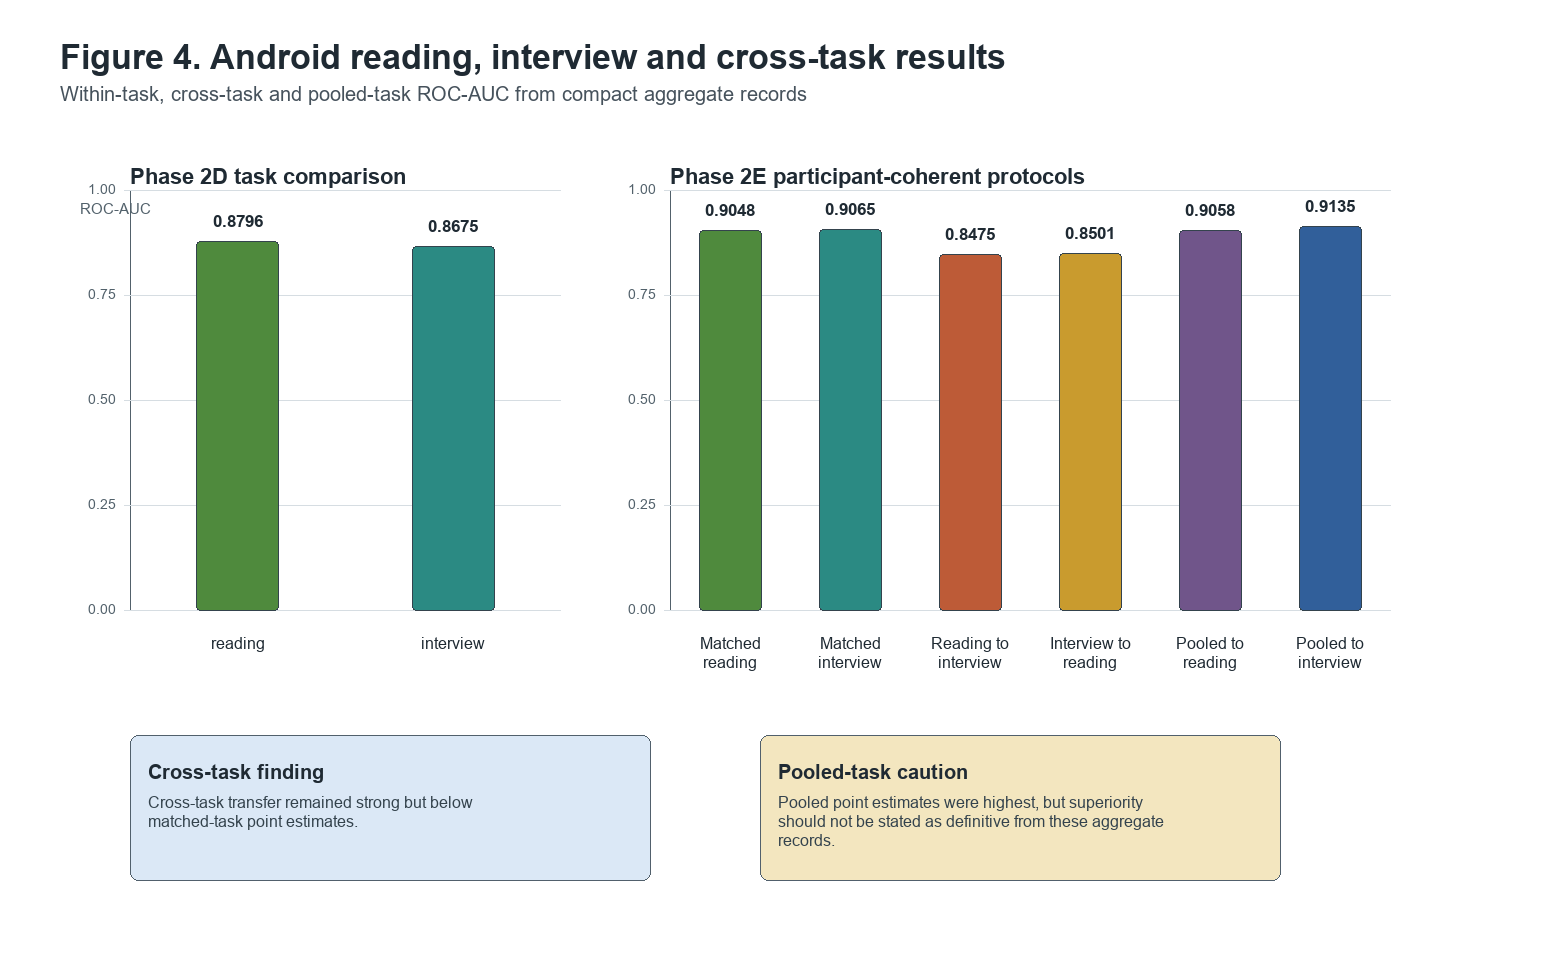
\includegraphics[width=0.95\textwidth]{figures/figure4_android_cross_task_results.png}
\caption{Android reading/interview task results and participant-coherent Phase 2E cross-task/pooled-task ROC-AUC values.}
\label{fig:android-cross-task}
\end{figure*}

\subsection{Participant-coherent cross-task transfer}

This experiment provides the controlled cross-task component of RQ4 by keeping paired reading and interview recordings from the same participant within the same fold.

Phase 2E used participant-coherent folds over 110 paired Android participants, with 52 HC and 58 PT participants. Matched within-task training achieved ROC-AUC 0.9048 for reading and 0.9065 for interview. Cross-task training remained strong but lower than matched-task training: reading-to-interview achieved ROC-AUC 0.8475, and interview-to-reading achieved ROC-AUC 0.8501. The reading-to-interview AUC gap versus matched interview was -0.0590, and the interview-to-reading gap versus matched reading was -0.0547.

Pooled reading-and-interview training achieved ROC-AUC 0.9058 for reading and 0.9135 for interview. Pooled-to-reading improved over interview-to-reading by 0.0557, and pooled-to-interview improved over reading-to-interview by 0.0660. However, the paired bootstrap intervals for these pooled gains included zero, so the pooled advantage should be interpreted as suggestive rather than conclusive.

\begin{table*}[!t]
\caption{Participant-coherent cross-task results}
\label{tab:cross-task}
\centering
\scriptsize
\setlength{\tabcolsep}{3pt}
\renewcommand{\arraystretch}{1.15}
\resizebox{\textwidth}{!}{%
\begin{tabular}{lllllllllll}
\toprule
Protocol & Source task & Target task & Participants & ROC-AUC & 95\% CI / comparison interval & PR-AUC & Brier & Balanced accuracy at 0.5 & Macro F1 at 0.5 & Interpretation \\
\midrule
Matched reading & Reading & Reading & 110 & 0.9048 & [0.8435, 0.9562] & 0.9281 & 0.1274 & 0.8273 & 0.8269 & Within-task reference \\
Matched interview & Interview & Interview & 110 & 0.9065 & [0.8452, 0.9589] & 0.9305 & 0.1214 & 0.8561 & 0.8545 & Within-task reference \\
Reading-to-interview & Reading & Interview & 110 & 0.8475 & AUC CI [0.7699, 0.9158]; gap [-0.1316, 0.0116] & 0.8877 & 0.2825 & 0.6867 & 0.6741 & Strong but below matched interview \\
Interview-to-reading & Interview & Reading & 110 & 0.8501 & AUC CI [0.7699, 0.9204]; gap [-0.1436, 0.0325] & 0.8602 & 0.1571 & 0.8176 & 0.8176 & Strong but below matched reading \\
Pooled-to-reading & Reading plus interview & Reading & 110 & 0.9058 & AUC CI [0.8442, 0.9539]; gain [-0.0172, 0.1340] & 0.9226 & 0.1232 & 0.8004 & 0.7997 & Suggestive gain; CI includes zero \\
Pooled-to-interview & Reading plus interview & Interview & 110 & 0.9135 & AUC CI [0.8515, 0.9635]; gain [-0.0013, 0.1346] & 0.9250 & 0.1122 & 0.8561 & 0.8545 & Suggestive gain; CI includes zero \\
\bottomrule
\end{tabular}%
}
\begin{minipage}{0.96\textwidth}
\vspace{2pt}
\footnotesize All rows are within the Androids Corpus. Pooled gains are suggestive because uncertainty intervals include zero.
\end{minipage}
\end{table*}


\subsection{Classifier-boundary analysis}

Phase 2E classifier-boundary analysis found only moderate similarity between reading-trained and interview-trained logistic-regression boundaries. Across folds, coefficient cosine similarity averaged 0.4752, coefficient sign agreement averaged 0.6659 and top-50 absolute-weight feature Jaccard overlap averaged 0.1216. Matched-task score correlation averaged 0.7123, while cross-target score correlation averaged 0.5555. These results support a distinction between shared representation information and partly task-specific classifier boundaries.

\begin{figure*}[!t]
\centering
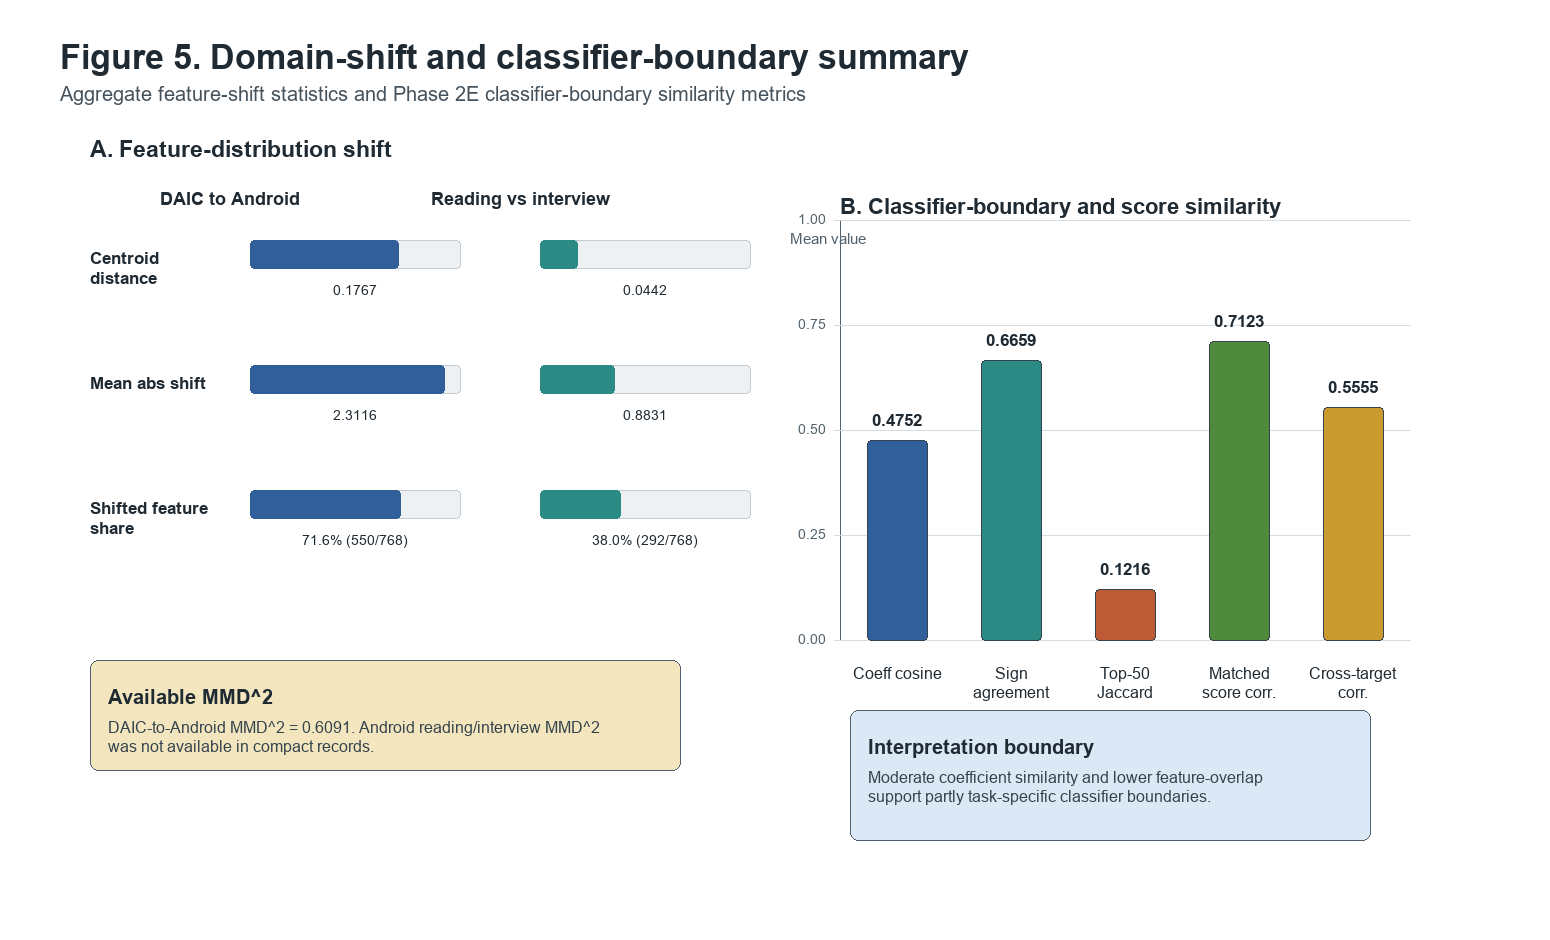
\includegraphics[width=0.95\textwidth]{figures/figure5_domain_shift_boundary_summary.png}
\caption{Aggregate domain-shift and classifier-boundary summaries. Panel A compares DAIC-to-Android feature shift with Android reading/interview task shift using centroid cosine distance, mean absolute standardized shift, shifted-feature share and available MMD\textsuperscript{2}. Panel B shows mean Phase 2E classifier-boundary and score-similarity metrics.}
\label{fig:domain-shift-boundary}
\end{figure*}

\begin{table*}[!t]
\caption{Result-scope and claim matrix}
\label{tab:result-scope}
\centering
\scriptsize
\setlength{\tabcolsep}{3pt}
\renewcommand{\arraystretch}{1.15}
\resizebox{\textwidth}{!}{%
\begin{tabular}{lllll}
\toprule
Result & Validation scope & Target-domain training? & External validation? & Allowed interpretation \\
\midrule
DAIC layer and aggregation development & Methodological ablation & No external target domain & No & Selects layer 9 and mean aggregation for later frozen representation use \\
DAIC Phase 1F WavLM Candidate A & Provisional local labeled DAIC test & No Android training & No & DAIC local labeled research estimate only \\
DAIC Phase 1F timing Candidate B & Provisional local labeled DAIC test & No Android training & No & Timing model works only under compatible guided-interview timing definitions \\
Phase 2B frozen DAIC-to-Android interview & Cross-corpus zero-shot external evaluation & No & Yes & Limited cross-corpus ranking transfer; thresholded classifier failed \\
Phase 2C threshold-only adaptation & Cross-corpus target adaptation & Threshold only & Yes, adapted & Threshold shift contributed to failure; not pure zero-shot \\
Phase 2C score calibration & Cross-corpus target adaptation & Calibration only & Yes, adapted & Calibration improved probability scale but not ranking \\
Phase 2C Android-trained interview & Within-corpus cross-validation & Yes & No & Strong within-Android interview discrimination with frozen WavLM features \\
Phase 2D Android-trained reading & Within-corpus cross-validation & Yes & No & Strong within-Android reading discrimination with frozen WavLM features \\
Phase 2E cross-task transfer & Cross-task transfer within Android & Yes, source task & No & Reading and interview share useful representation information, with task-specific boundaries \\
Phase 2E pooled-task training & Pooled-task within Android & Yes & No & Highest point estimates; pooled gains suggestive because intervals included zero \\
\bottomrule
\end{tabular}%
}
\begin{minipage}{0.96\textwidth}
\vspace{2pt}
\footnotesize This matrix preserves the distinction between methodological ablations, provisional local testing, zero-shot external evaluation, target-domain adaptation and within-corpus validation.
\end{minipage}
\end{table*}


\section{Discussion}

\subsection{Main findings}

The experiments support three main findings. First, frozen WavLM layer-9 representations contained depression-related ranking information across corpora and tasks. Second, direct transfer of the DAIC-trained classifier failed at the threshold and probability-scale level, especially on Android interview and reading speech where all zero-shot thresholded predictions were negative. Third, target-corpus classifier learning and pooled task exposure substantially improved discrimination within Android.

\subsection{Findings in Relation to the Research Questions}

For RQ1, the DAIC-WOZ experiments showed that frozen WavLM representations provided weak-to-modest participant-level discrimination, while guided-interview timing features produced stronger local labeled-test performance but were not directly portable to Android because compatible timing annotations were incomplete. For RQ2, layer selection and participant aggregation influenced the DAIC development pipeline: layer 9 was retained over the final layer, and mean aggregation was kept because alternative aggregation strategies did not improve the DAIC train-only comparisons. For RQ3, DAIC-to-Android transfer preserved some ranking signal but failed as direct thresholded classification; target-domain threshold adaptation, score calibration and Android-trained classifiers showed that probability scale and classifier-boundary shift were central limitations. For RQ4, Android reading and interview speech shared useful representation information, but task condition still mattered: matched-task and pooled-task models were strongest within Android, while cross-task transfer remained below matched-task training and classifier boundaries were only moderately similar.

Because WavLM representations may encode speaker-specific information together with behavioral cues, these experiments should not be interpreted as having disentangled depression markers from biometric voice characteristics. Dedicated speaker-disentanglement or adversarial-invariance experiments would be required to test that question directly.

\subsection{Representation transfer versus classifier transfer}

The contrast between zero-shot ROC-AUC and thresholded predictions is central. A ROC-AUC of 0.6412 on Android interview speech showed that the frozen DAIC scores ranked PT participants above HC participants more often than chance. Yet the same score distribution lay entirely below the frozen decision thresholds. This means the representation-score combination contained some ranking signal, but the source-trained probability scale and classifier boundary did not transfer sufficiently for direct thresholded use. This distinction follows the calibration literature's separation between discrimination and the reliability of predicted probabilities \cite{niculescuMizil2005probabilities,vanCalster2019calibration}.

\subsection{Corpus-specific decision boundaries}

The domain-shift analysis suggests that the main limitation was not simply threshold choice. Threshold adaptation improved macro F1, and calibration improved Brier score, but the Android-trained classifier produced the largest discrimination improvement. The 550 shifted WavLM features and the 0.2263 AUC gain from Android classifier training are consistent with corpus-specific decision boundaries. Here, classifier-boundary shift is used descriptively: it means that a new target-domain logistic-regression boundary on the same frozen features separated Android HC/PT participants much better than the DAIC-trained boundary. This interpretation is aligned with broader observations that dataset shift can affect feature distributions, class priors, conditional relationships and classifier calibration \cite{morenoTorres2012datasetShift,vanCalster2019calibration}.

\subsection{Reading and interview speech}

Reading speech and interview speech produced similar within-Android discrimination when each task had its own classifier. Prior speech-depression literature treats task design as a meaningful source of variation: reading can control lexical content and topic variability, while interviews preserve spontaneous fluency, conversational timing and response structure \cite{tao2023androids,tao2023featureCorrelation,leal2025survey}. The high within-participant representation similarity in this study suggests shared acoustic or vocal information across tasks. At the same time, cross-task transfer was weaker than matched-task training, and classifier coefficients showed only moderate similarity. Reading and interview tasks therefore appear to share useful representation structure while still requiring partly task-specific classifier boundaries.

\subsection{Benefits and limits of pooled-task learning}

Pooled reading-and-interview training produced the strongest point estimates in Phase 2E. Pooled-to-reading ROC-AUC was 0.9058 and pooled-to-interview ROC-AUC was 0.9135. These gains are consistent with the idea that exposure to both tasks can help the classifier learn a more robust boundary. However, the paired bootstrap intervals for pooled gains included zero, so the pooled advantage should be described as suggestive, not definitive.

\subsection{Implications for cross-corpus depression detection}

The results argue for careful protocol labeling in cross-corpus depression detection. A zero-shot external evaluation, a target-domain threshold adaptation, a target-domain calibration and a within-corpus trained classifier answer different questions. The Android-trained interview and reading results demonstrate strong within-corpus discrimination with frozen WavLM features, but they do not prove direct DAIC-to-Android model transfer. Conversely, the DAIC zero-shot results show limited external ranking transfer but not clinically usable thresholded performance. Prior cross-corpus depression-speech work makes this distinction important because transfer settings can mix language, task, label-source and recording changes rather than isolating one cause \cite{alghowinem2016crossCultural,seneviratne2021generalized,leal2025survey}.

\subsection{Comparison with prior work}

The findings are broadly consistent with prior concerns that depression speech models can be sensitive to dataset, task and language differences \cite{alghowinem2016crossCultural,seneviratne2021generalized,leal2025survey}. They also align with the expectation that self-supervised representations provide useful general speech features, while downstream classifiers require careful validation under target conditions \cite{baevski2020wav2vec2,yang2021superb,wu2023sslDepression,huang2024voicePretraining}. These sources support the methodological comparison, but they do not imply that this study has established clinical deployment readiness or domain-invariant depression biomarkers.

\section{Ethical and Clinical Considerations}

These are research-only classification results. They do not establish clinical diagnosis, screening utility or deployment readiness. The models are not diagnostic tools. DAIC-WOZ PHQ8\_Binary labels and Android HC/PT labels were supervisory labels for model evaluation, not clinical endpoints validated prospectively in this study. Adult depression-screening guidance assumes further diagnostic evaluation and adequate systems for treatment and follow-up, so a speech classifier should not be interpreted as a stand-alone diagnostic pathway \cite{uspstf2023depressionScreening}.

Speech data are also sensitive because voice can contain information about identity, language, accent, health, emotion and recording environment. Speech-data governance should therefore address consent, access control, retention, data minimization, de-identification limits and voice re-identification risk \cite{nautsch2019gdprSpeech,tomashenko2021voicePrivacy}. The present repository excludes raw audio, embeddings, participant predictions and fitted models from versioned paper artifacts, and the compact registry records are designed for auditability without redistributing restricted speech data.

Bias and fairness remain open requirements. The corpora differ in language, recruitment, task design and label source, and the study did not perform subgroup evaluation by sex, age, dialect, accent, site or other demographic variables. Prior speech-technology evidence shows that automated speech systems can have differential performance across speaker groups, and the NIST AI RMF treats harmful-bias management, privacy, validity, reliability, safety, transparency and accountability as core trustworthy-AI concerns \cite{koenecke2020racialDisparitiesASR,nist2023aiRmf}. No demographic fairness audit was completed.

Clinical deployment would require evidence beyond the retrospective experiments reported here. Prospective or early-stage clinical evaluation should examine actual clinical performance, safety, human factors, error modes, workflow fit, local representativeness, calibration in the target population and downstream patient outcomes \cite{kelly2019clinicalImpactAI,vasey2022decideAI,liu2020consortAI,vanCalster2019calibration}. No prospective deployment study was performed. No clinical utility study was completed. Any future use should include human oversight, locally validated thresholds, monitoring for distribution shift, clear escalation pathways and governance for updates or decommissioning \cite{who2021aiHealthEthics,nist2023aiRmf}.

\section{Limitations}

The study had several limitations. Dataset sizes were modest, especially for participant-level cross-validation. DAIC-WOZ and Androids Corpus used related but non-identical target labels: PHQ-8 binary labels in DAIC and clinical group status in Android. The corpora differed in language, recording conditions, task structure and participant recruitment. The Phase 1F DAIC test labels were from a local labeled file without established official hidden AVEC provenance. Android-trained models were not evaluated on an independent third corpus. Phase 2D reading and interview comparisons were initially descriptive because original task folds differed; Phase 2E addressed this with participant-coherent folds but remained within Androids Corpus. No demographic fairness analysis, subgroup calibration study, uncertainty-aware clinical threshold study, prospective validation, workflow evaluation or clinical utility study was performed. The models were not compared with clinician assessment at the point of care. False positives and false negatives were not evaluated in a clinical workflow, and the appropriate actionability of any threshold remains unknown. The privacy analysis was limited to documentation and artifact exclusion rather than a formal governance review. The adaptation comparisons intentionally used logistic regression only, so they do not address whether more complex model families would improve performance. Finally, the confidence intervals for pooled-task gains included zero, so pooled-task superiority was not definitively established.

\section{Conclusion}

This study addressed four questions about frozen speech representations, DAIC-WOZ development choices, DAIC-to-Android transfer and Android task effects. The results indicate that speech representations and timing descriptors can encode depression-related behavioral signal, but DAIC performance was sensitive to the feature family and the strongest timing model was not directly transferable to Android. WavLM layer and aggregation choices also shaped the selected DAIC pipeline. Across corpora, the DAIC-trained WavLM classifier retained limited ranking information but did not transfer as a thresholded classifier, showing the importance of calibration, threshold and classifier-boundary analysis. Within Android, reading and interview speech shared information but remained partly task-specific, with pooled-task gains interpreted cautiously. These findings support research on representation transfer and corpus-specific calibration, not clinical readiness. External validation beyond Androids Corpus, demographic fairness evaluation, privacy governance, prospective clinical validation and clinical utility assessment remain necessary before any clinical claim can be made.

\section{Data and Code Availability}

The source datasets are not redistributed. Access to DAIC-WOZ and Androids Corpus data remains governed by the original dataset terms \cite{gratch2014distress,valstar2016avec,tao2023androids}. The repository preserves code, compact configuration records, paper evidence maps and the experiment registry associated with the frozen source tag \texttt{paper-experiment-freeze-v1}. Raw audio, participant-level artifacts, embeddings, fitted models and participant predictions are excluded from the paper artifacts because they may contain restricted or sensitive information. This supports auditability of reported claims while limiting third-party reproduction of restricted-data processing to users who separately obtain the underlying datasets under their original access conditions.

\section*{Acknowledgment}
The authors thank the creators and maintainers of the DAIC-WOZ and Androids Corpus datasets. Mohammad Ilyas acknowledges the academic guidance received during his Ph.D. research work.

\section*{Funding}
No funding was received for this study.

\section*{Competing Interests}
The authors declare no competing interests.

\section*{Ethics Approval}
This study used previously collected datasets obtained under their original access terms. No new human participants were recruited. Ethics approval was not sought because the study involved secondary analysis of existing datasets.

\section*{Consent to Participate}
This study used secondary datasets obtained under their original access terms. Consent for the original data collection was managed by the respective dataset providers. No new human participants were recruited in this study.

\section*{Consent for Publication}
This study used secondary datasets obtained under their original access terms. Consent for the original data collection was managed by the respective dataset providers. No new human participants were recruited in this study.

\section*{Author Contributions}
Mohammad Ilyas: Conceptualization, Methodology, Software, Validation, Formal analysis, Investigation, Data curation, Writing - original draft, Visualization, Project administration.

Dr. Vikram Singh: Supervision.

\section*{Declaration of Generative AI and AI-Assisted Technologies in the Writing Process}
ChatGPT and Codex were used to assist with code organization, manuscript drafting support, editing, and workflow planning. The authors reviewed and verified the manuscript content, results, references, and final scientific claims.

\section*{Preprint Statement}
A preprint is planned.


\bibliographystyle{IEEEtran}
\bibliography{bib/references}

\begin{IEEEbiography}{Mohammad Ilyas}
[AUTHOR CONFIRMATION REQUIRED: IEEE biography]
\end{IEEEbiography}

\begin{IEEEbiography}{Vikram Singh}
[AUTHOR CONFIRMATION REQUIRED: IEEE biography]
\end{IEEEbiography}

\end{document}
